\subsection{Other Negative Parity Bands}
\subsubsection{K$^\pi$=5$^-$ Band}
The current status/insight of this K$^\pi$=5$^-$ band is of a two-quasiparticle origin \cite{Aprahamian200642}, where we can verify this interpretation with the (albeit slightly inflated at $\sim$0.3~mWu) weak E1 transition strengths to the ground state. Furthermore, K$^\pi$=5$^-$ bands are not surmised to be a part of the octupole vibration splitting in a deformed nucleus, yet the refinement of this lifetime from older literature values is important nonetheless.

Assertions from IBM considerations with the inclusion of \textit{p} and \textit{f} bosons imply that the structure of the lowest-lying negative parity bands may not be of purely collective nature  \cite{Aprahamian200642, Iachello_Arima_IBM}, where the traditional picture of octupole collectivity in well-deformed nuclei exists with the initial, lowest-lying and fragmented quartet of states of K$^\pi$=0$^-$, 1$^-$, 2$^-$, \& 3$^-$. However, the current ordering of negative parity bands in $^{162}$Dy is difficult (read: impossible) to predict with modern models \cite{Aprahamian200642}. Lifetimes for a few other of the lowest-lying set of states in $^{162}$Dy have been measured, and individual discussion of the measurements is provided below.

\subsubsection{K$^\pi$=3$^-$ Band}
This creates a somewhat murky picture for any interpretation of the K$^\pi$=3$^-$ band. The E$_\gamma$=311~keV de-excitation from the 4$^-$ member is overwhelmingly E2 radiation, based on our measurement of a mixing ratio of -6.9$^{+1.6}_{-2.2}$ ($\sim$98\% E2), but the very large (potentially) E2 transition probabilities that de-excite the bandhead are impressive, even in the face of heavy M1 mixing for the 212~keV $\gamma$ ray that leaves the bandhead at 1570~keV. Whether this band is some higher collective behavior on top of the existing octupole vibration or if it is even part of the 0$^-$, 1$^-$, 2$^-$, 3$^-$ quartet is still an open question, however, the preference of decay to the lower-lying octupole band (K$^\pi$=0$^-$ band) should not be understated.
% K=3- band could be a double octupole, with strong preference to decay to the k=0-, really, this breaks the notion that the lowest-lying neg parities are the fragmented octupole
\subsubsection{K$^\pi$=1$^-$ Band}

As such, the deduced transition probabilities should not be taken without careful attention and heavy skepticism. Interband B(E2) strengths of 630~W.u. are unprecedented in \textit{any} nuclear transition, flagging a clear departure from a consistent measurement of the lifetime. The generally low limits for lifetimes measured do not offer vast insight into the collectivity of the band.
%do an ExF for the 1739 state here too



% we observe remarkably strong B(E2)s to the 2$^-$ band, even considering the large uncertainties and heavy E2/M1 mixing to the bandhead of the 2$^-$ band. The full energy de-excitation to the ground state exhibits a very non-collective E1 transition, immediately pointing away from a single-octupole picture. The 1691~keV state follows in line with the bandhead, with a strong B(E2) to the 2$^-$ band with high M1-mixing and a somewhat suppressed transition probability to ground state. Mixing information was not extracted for the 416~keV $\gamma$ ray to the 0$^-$ octupole band, so the quoted B(E2) value in Table \ref{tab:162Dy_negparity_low} is essentially an upper limit. Yet again, in the 3$^-$ member of the band, we observe strong E2 radiation to the 2$^-$ band (the 529~keV $\gamma$ ray is $\sim$100\% M1 radiation), with suppression of B(E1)s to the $\gamma$ and ground state band. Qualitatively, this suggests some strong quadrupole collectivity built on top of the 2$^-$ band in $^{162}$Dy; this deduction and decay pattern is in stark contrast to the simple picture of octupole collectivity in deformed nuclei, where the lowest quartet of negative parity states arise from the single $\lambda$=3 phonon fragmentation. Nearby rare-earth nuclei ($^{168}$Er) display strong E3 transition probabilities, with suppressed intraband B(E1)s [REFS], making $^{162}$Dy an anomaly in this sense. From our measurement of lifetimes and $\gamma$-ray spectroscopy, the question on the existence of this traditional picture of octupole collectivity seems tentative, with the existence of strong electric dipole transitions to the $\gamma$-vibrational band and to lower-lying negative parity states.


% \subsection{Higher Lying K$^\pi$=5$^-$, 3$^-_2$, 2$^-_2$ Bands}

\subsubsection{K$^\pi$=3$^-_2$ Band}
Decays from the second K$^\pi$=3$^-$ band have the potential for some interesting structure effects, with the extremely preferential branching ratios to the $\gamma$-band and the K$^\pi$=2$^-$ band. However, measurements of the second K$^\pi$=3$^-$ band's lifetimes cannot reveal any insight to the octupole collectivity in these levels.  In the case of mostly E2 radiation and the lowest possible lifetime, the alarmingly large B(E2)$\sim$6~Wu to the 2$^-$ band could indicate some collectivity on top of the K$^\pi$=2$^-$ octupole band, based solely on the decay pattern, but nothing concrete can be said, barring a reliable measurement of the actual lifetime of the states in the band.

% The measurement of the single lifetime limit for the bandhead of the 4$^-$ is taken from the only de-excitation observed in a  E$_\gamma$=327~keV decay to the K$^\pi$=4$^+$ bandhead. Negative parity lifetimes were measured using the GRID technique by Aprahamian (unpublished work); the range of lifetimes measured in that experiment for the 1862~keV level are in excellent agreement with our limit (1580-2860~fs). (This same argument also applies to our measurement of the lifetime for the 5$^-$ state at 1485~keV, which was given an upper limit of 2910~fs from the Doppler broadening technique.) Using this range of lifetimes from GRID, we are presented with a much clearer picture on the collectivity of this state at 3.3-5.9~mWu strength for the decay to the 4$^+$ band. This rather enhanced B(E1) suggests the idea that there could be some definite octupole collectivity built on top of the K$^\pi$=4$^+$ band. 

\begin{landscape}
\begin{figure}[h!]
\begin{center}
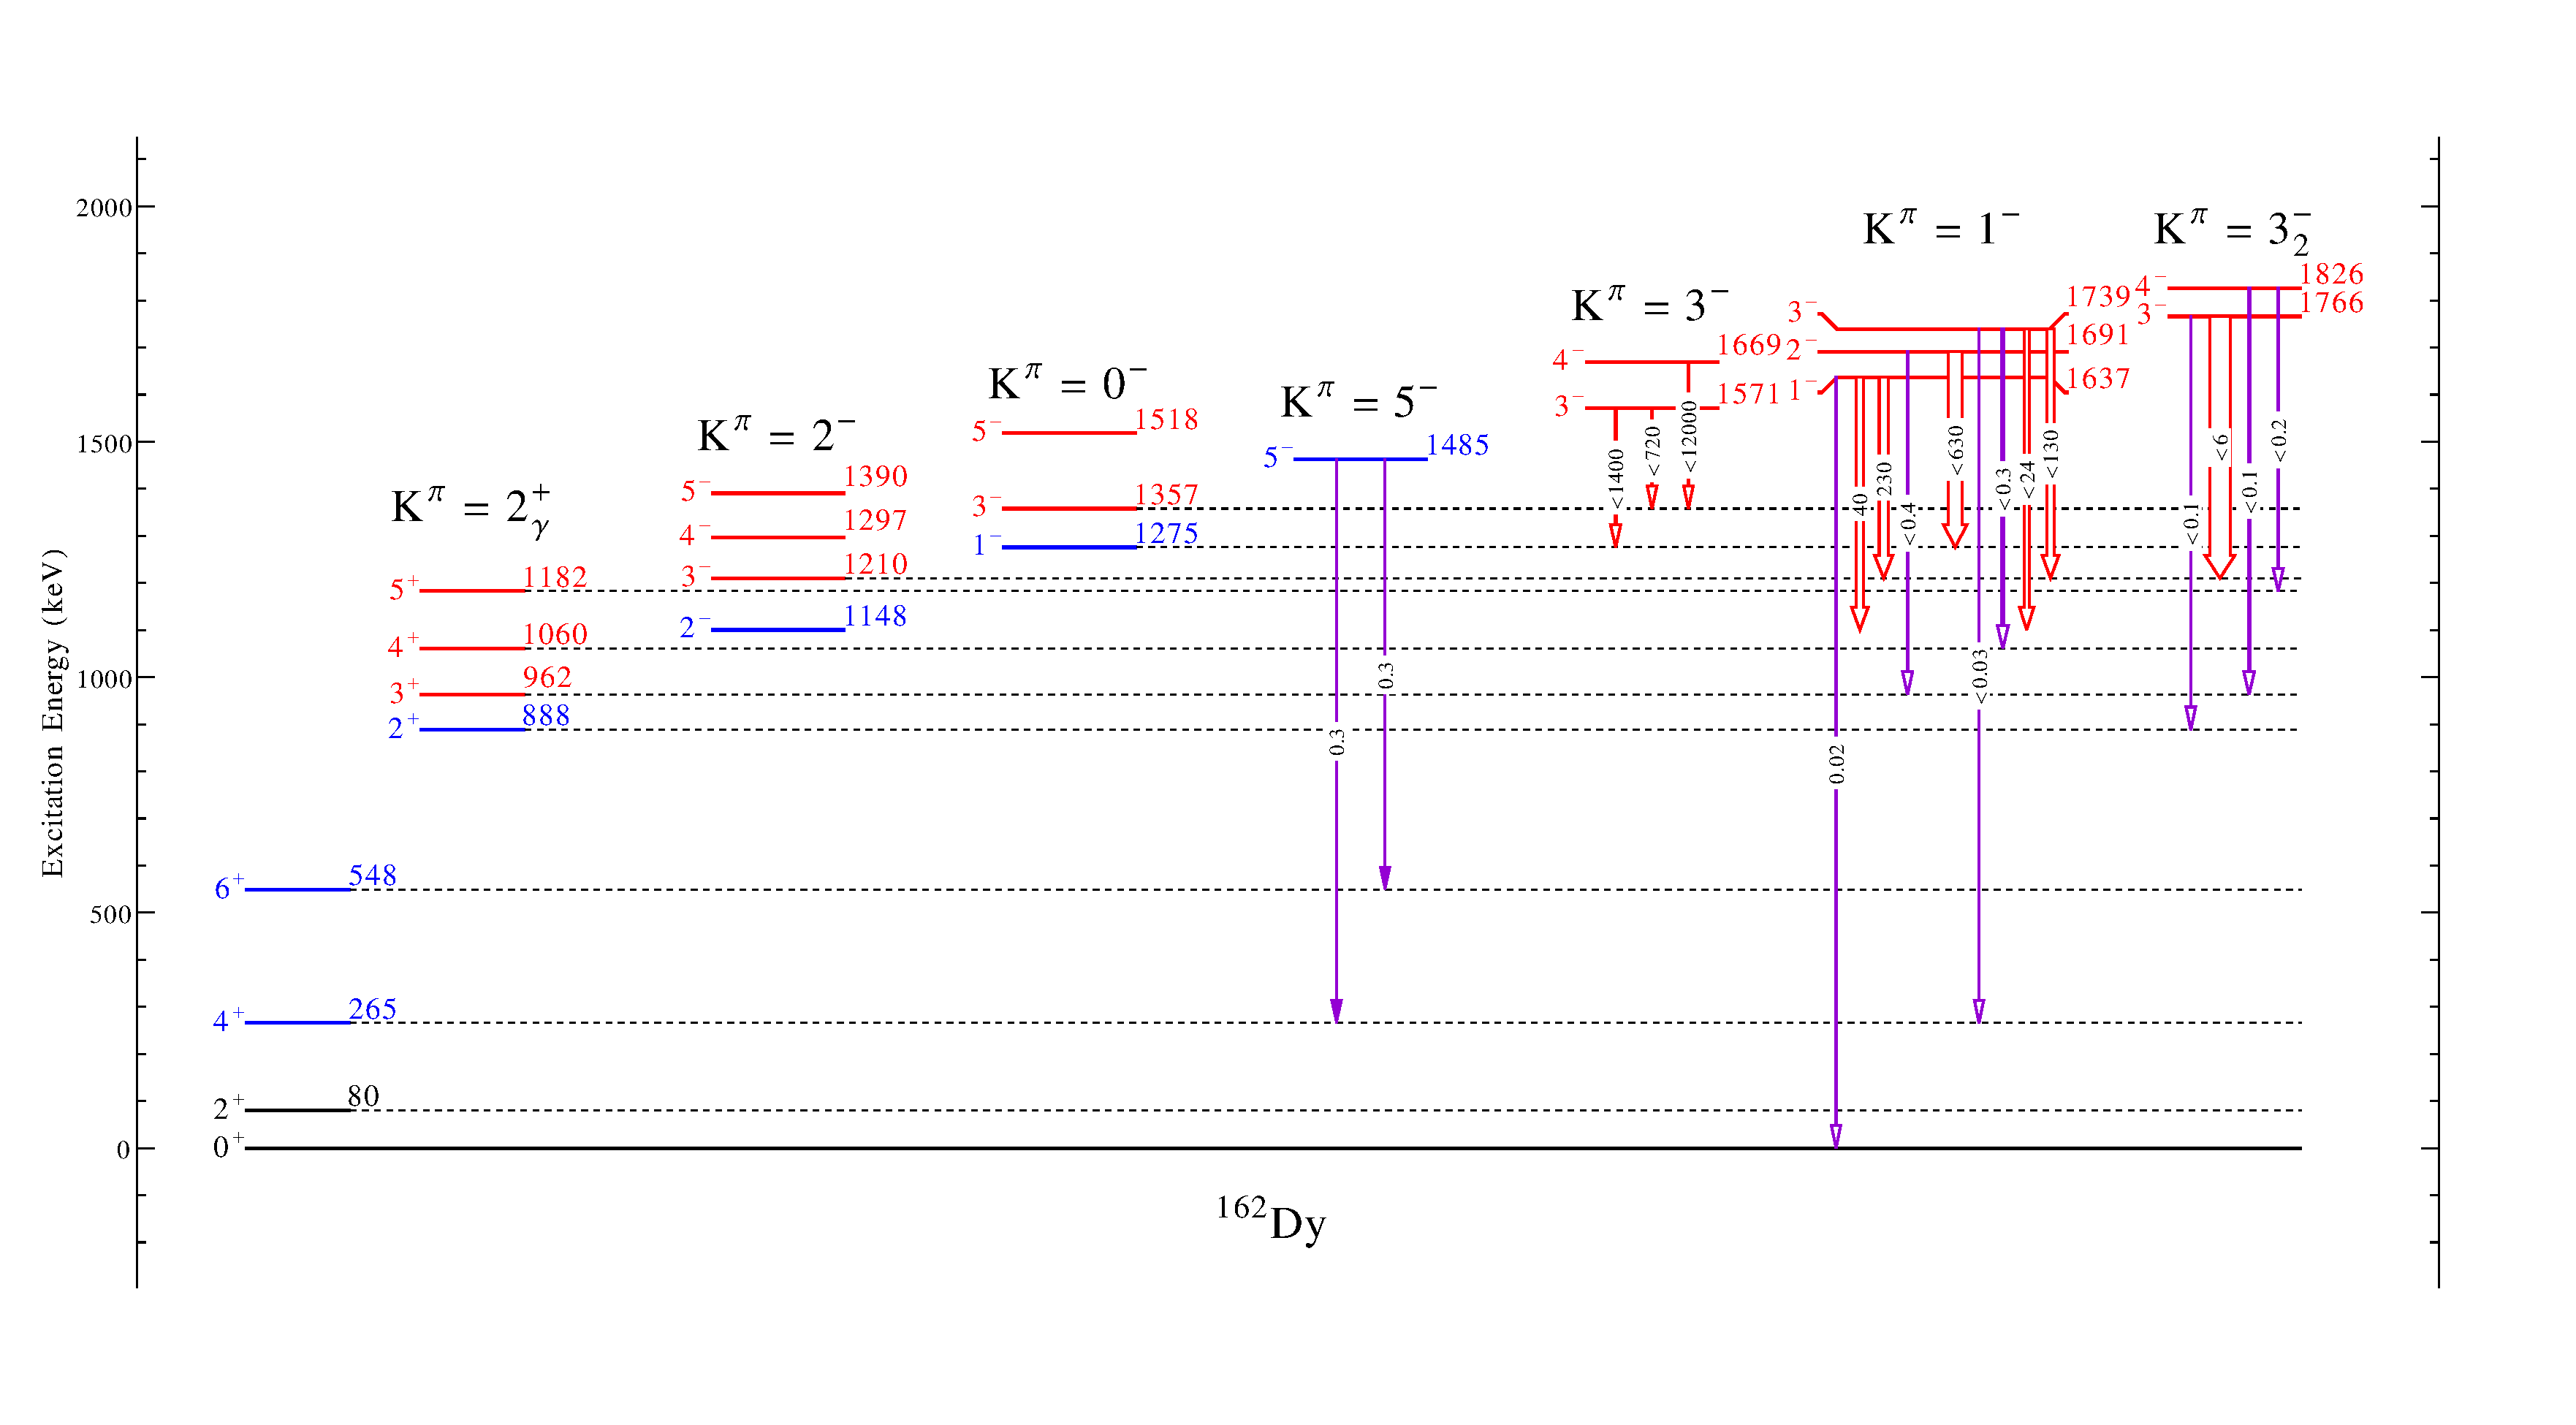
\includegraphics[height=0.85\textheight]{figures/162Dy_otherNeg.pdf}
\caption{Observed $\gamma$-decays from higher lying K$^\pi$=5$^-$, 3$^-$, 1$^-$, 3$^-_2$ bands in $^{162}$Dy. Transition strengths are proportional in width, with E2 transitions in red and E1 transitions in violet (color online). Hollow (white with colored border) transition arrows indicate that the resulting transition probability is tentatively from an unreliable lifetime measurement. \label{fig:162Dy_highbands}}
\end{center}
\end{figure}
\end{landscape}

\subsection{K$^\pi$=1$^+$ Band}
In terms of rotational bands in $^{162}$Dy, the discussion on results ends with the K$\pi$=1$^+$ band and the isovector M1 scissors mode. The latter excitations have been extensively studied with photon scattering experiments by \cite{Margraf_gg'NRF_1995,Yates_162nnp1995}, and as mentioned before, offer a good calibration point or benchmark for our lifetime measurements, as the literature values fall within the sensitive range of what DSAM can measure. 


At higher energies in this band, more channels are open to decay, which can be seen in Figure \ref{fig:162Dy_scissors}. While a fairly collective transition was measured to the $\gamma$-vibrational band, this should be taken as the exception to the rule, rather than implying that it is any collective behavior built on top of the existing quadrupole vibration. Oftentimes, a state can pick up a large two-quasiparticle amplitude from the `daughter' state that would give rise to a nonzero B(E2), however, this does not mean the state is collective in nature.

Overall, these transitions observed out of the 1$^+$ band are noncollective to any other excitation in $^{162}$Dy, an assertion made very early by Soloviev \cite{Solovev_162K2octupole}, suggesting that the K$^\pi$=1$^+$ band cannot stem from one or two-phonon coupling from the detailed quasiparticle-phonon nuclear model (QPNM) formalism outlined there.  

\begin{figure}[h!]
\begin{center}
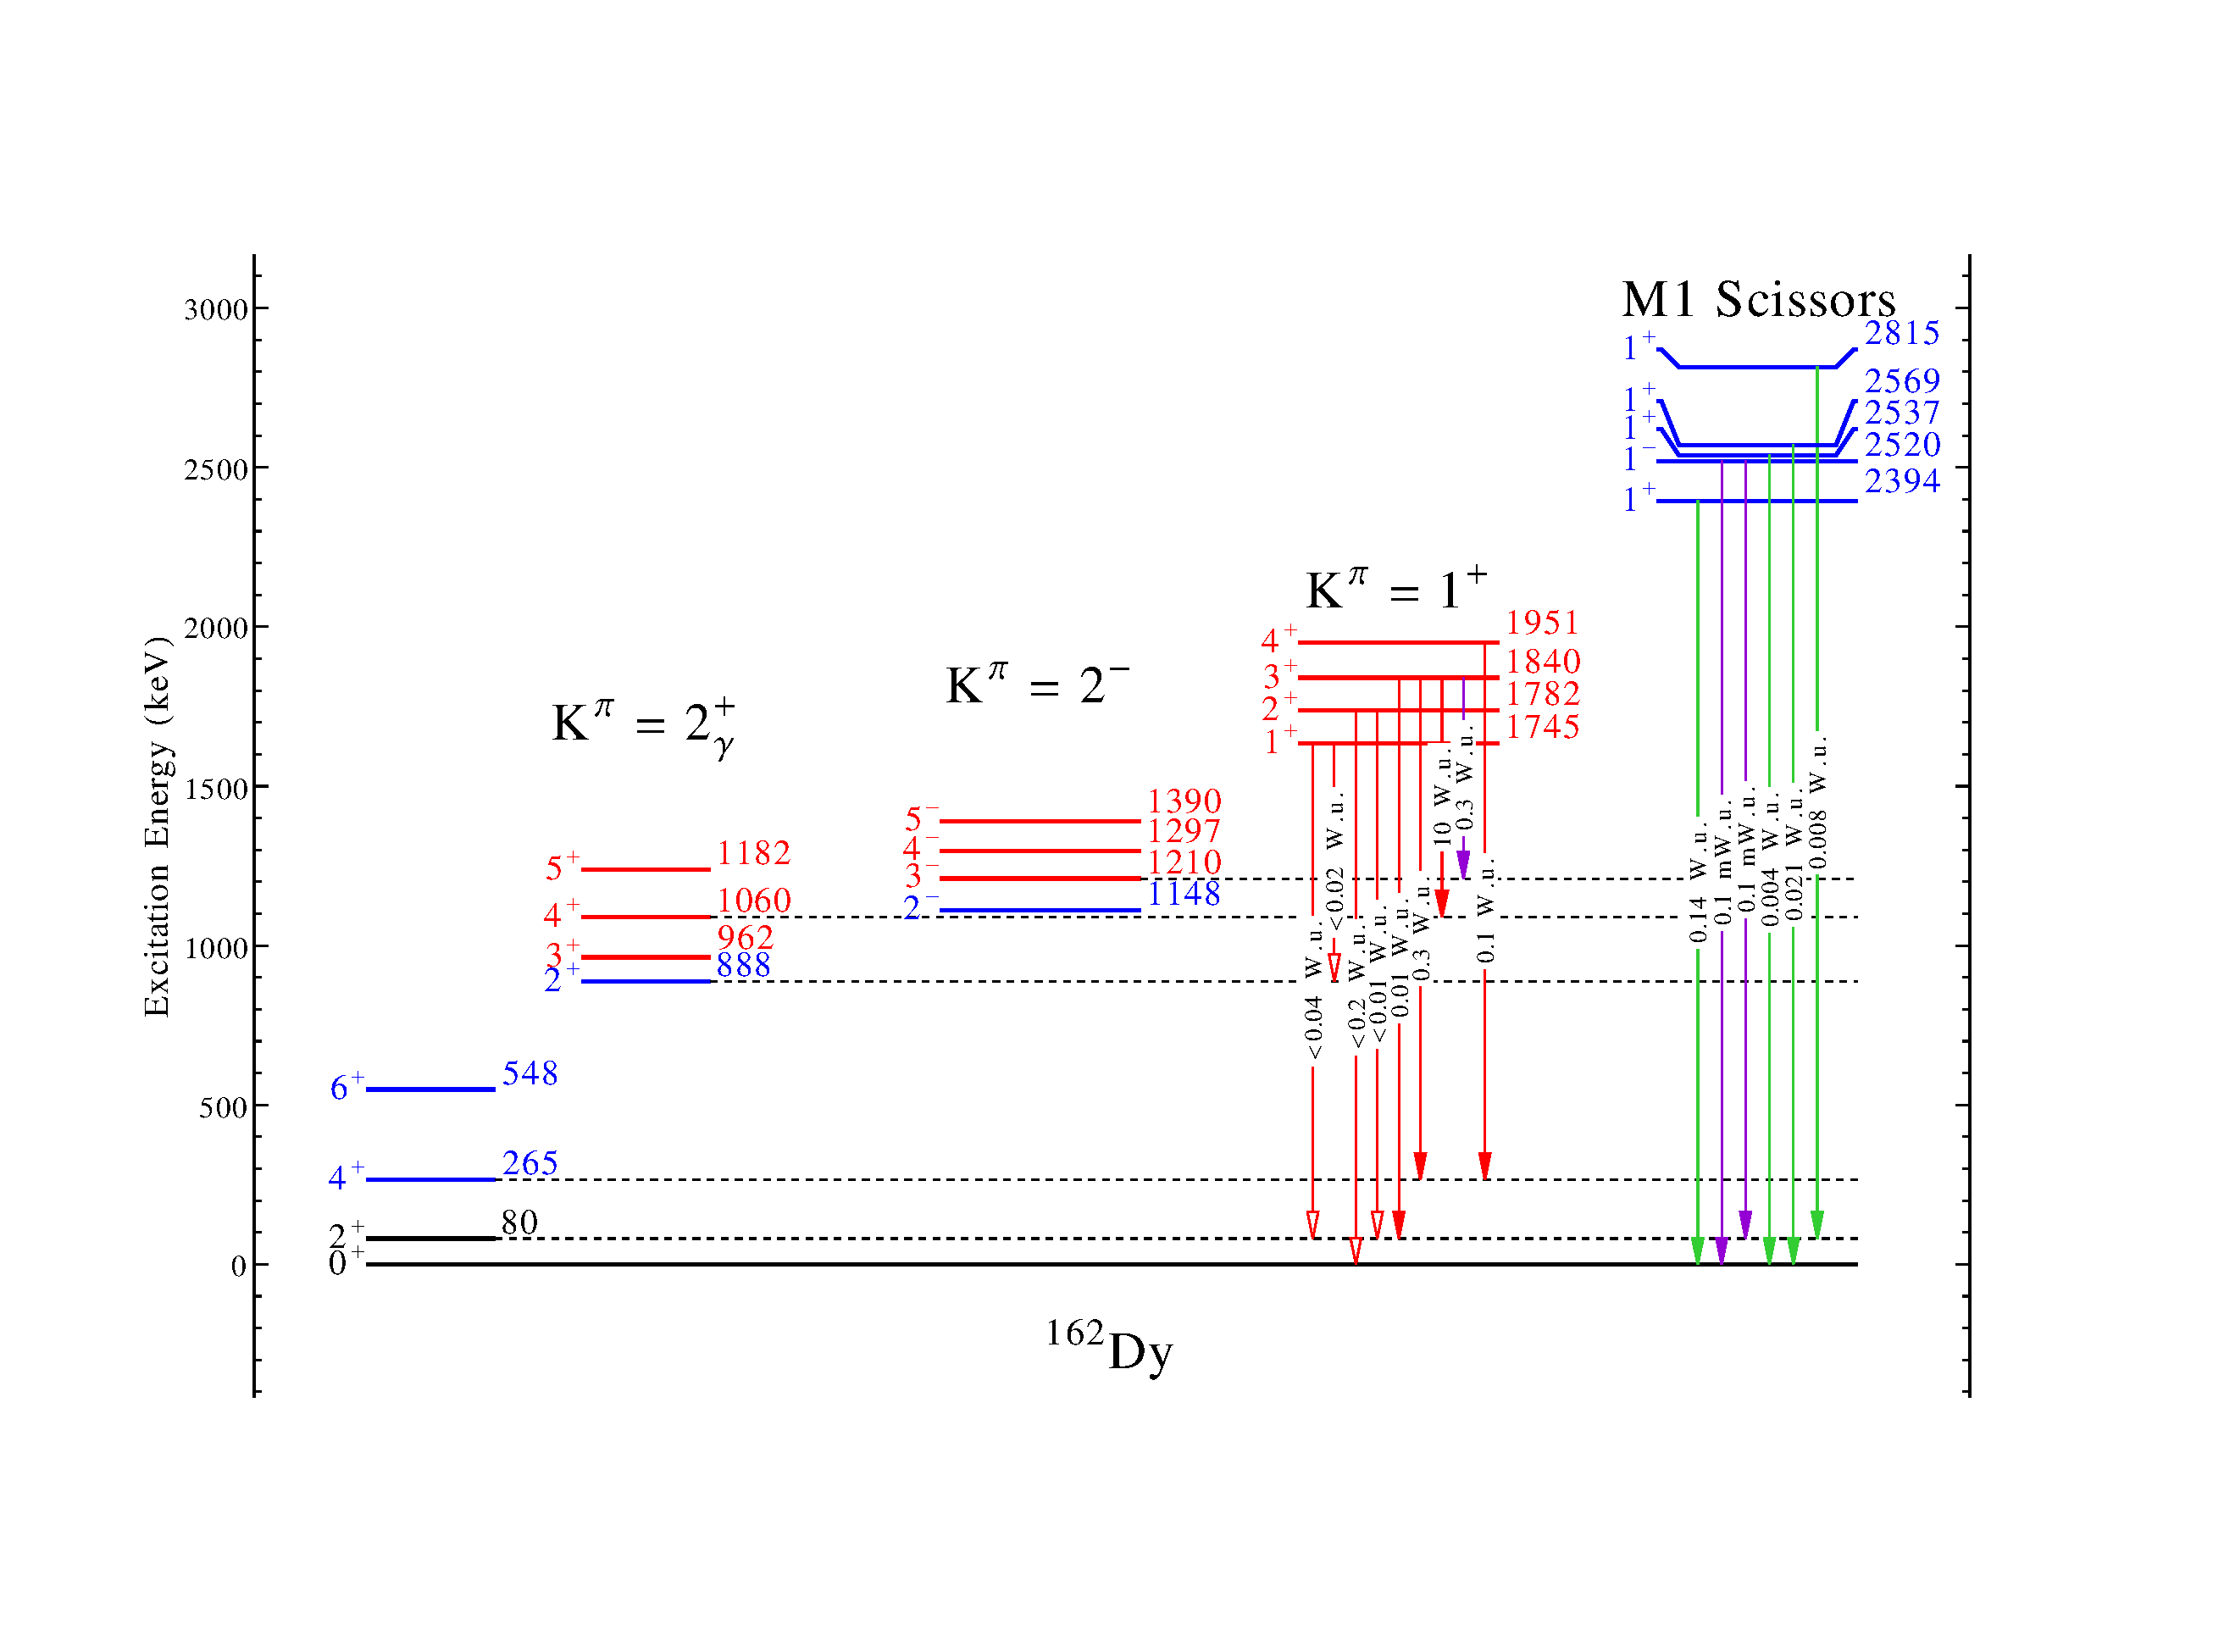
\includegraphics[width=0.97\textwidth]{figures/162Dy_scissors.pdf}
\end{center}
\caption{K$^\pi$=1$^+$ band and the 1$^\pm$-spin levels part of the isovector M1 scissors mode in $^{162}$Dy. B(E1) in violet and in mW.u., B(M1) in green and W.u., and B(E2) in red in W.u. \label{fig:162Dy_scissors}}
\end{figure}
\subsection{States Above 2.2~MeV Excitation Energy}
With the increasing level density and uncertainty in spin-parity assignments above 2.0~MeV, differentiation of negative parity bands (or \textit{any} band structure) becomes difficult. Incidentally, levels above this energy threshold lie well above the pairing gap; recall that we are most likely to find the most collective excitations below this energy, however, above the pairing gap, we can expect to see mixing between multi-quasiparticle states and collective excitations. Since the nature and goal of (n,n$^\prime\gamma$) experiments at UKAL is \textit{not} to identify new levels in the level scheme, but to confidently place existing $\gamma$-rays from the excitation functions, higher-lying states often cannot be confidently discussed in the scope of a vibrational phonon picture in this work. Of course, this does not imply that there is a lack of structure above this threshold, as we can observe multiphonon excitations at energies above the pairing gap \cite{Zamfir_doubleoctupole_2002, WuAprahamian_multiphonon_1994}. Reduced transition probabilities for transitions out of these states should not be given much weight, as a) the full E2 strength is reported for any potentially mixed multipolarity decays, and b) the E$_\gamma^{2\ell+1}$ factor for the calculation of reduced transition probabilites tends to dominate at this higher energy regime. Nevertheless, our measured lifetimes are presented and any observed branching ratios from multi-channel decays in the tables.

\begin{landscape}
\begin{figure}[h!]
\begin{center}
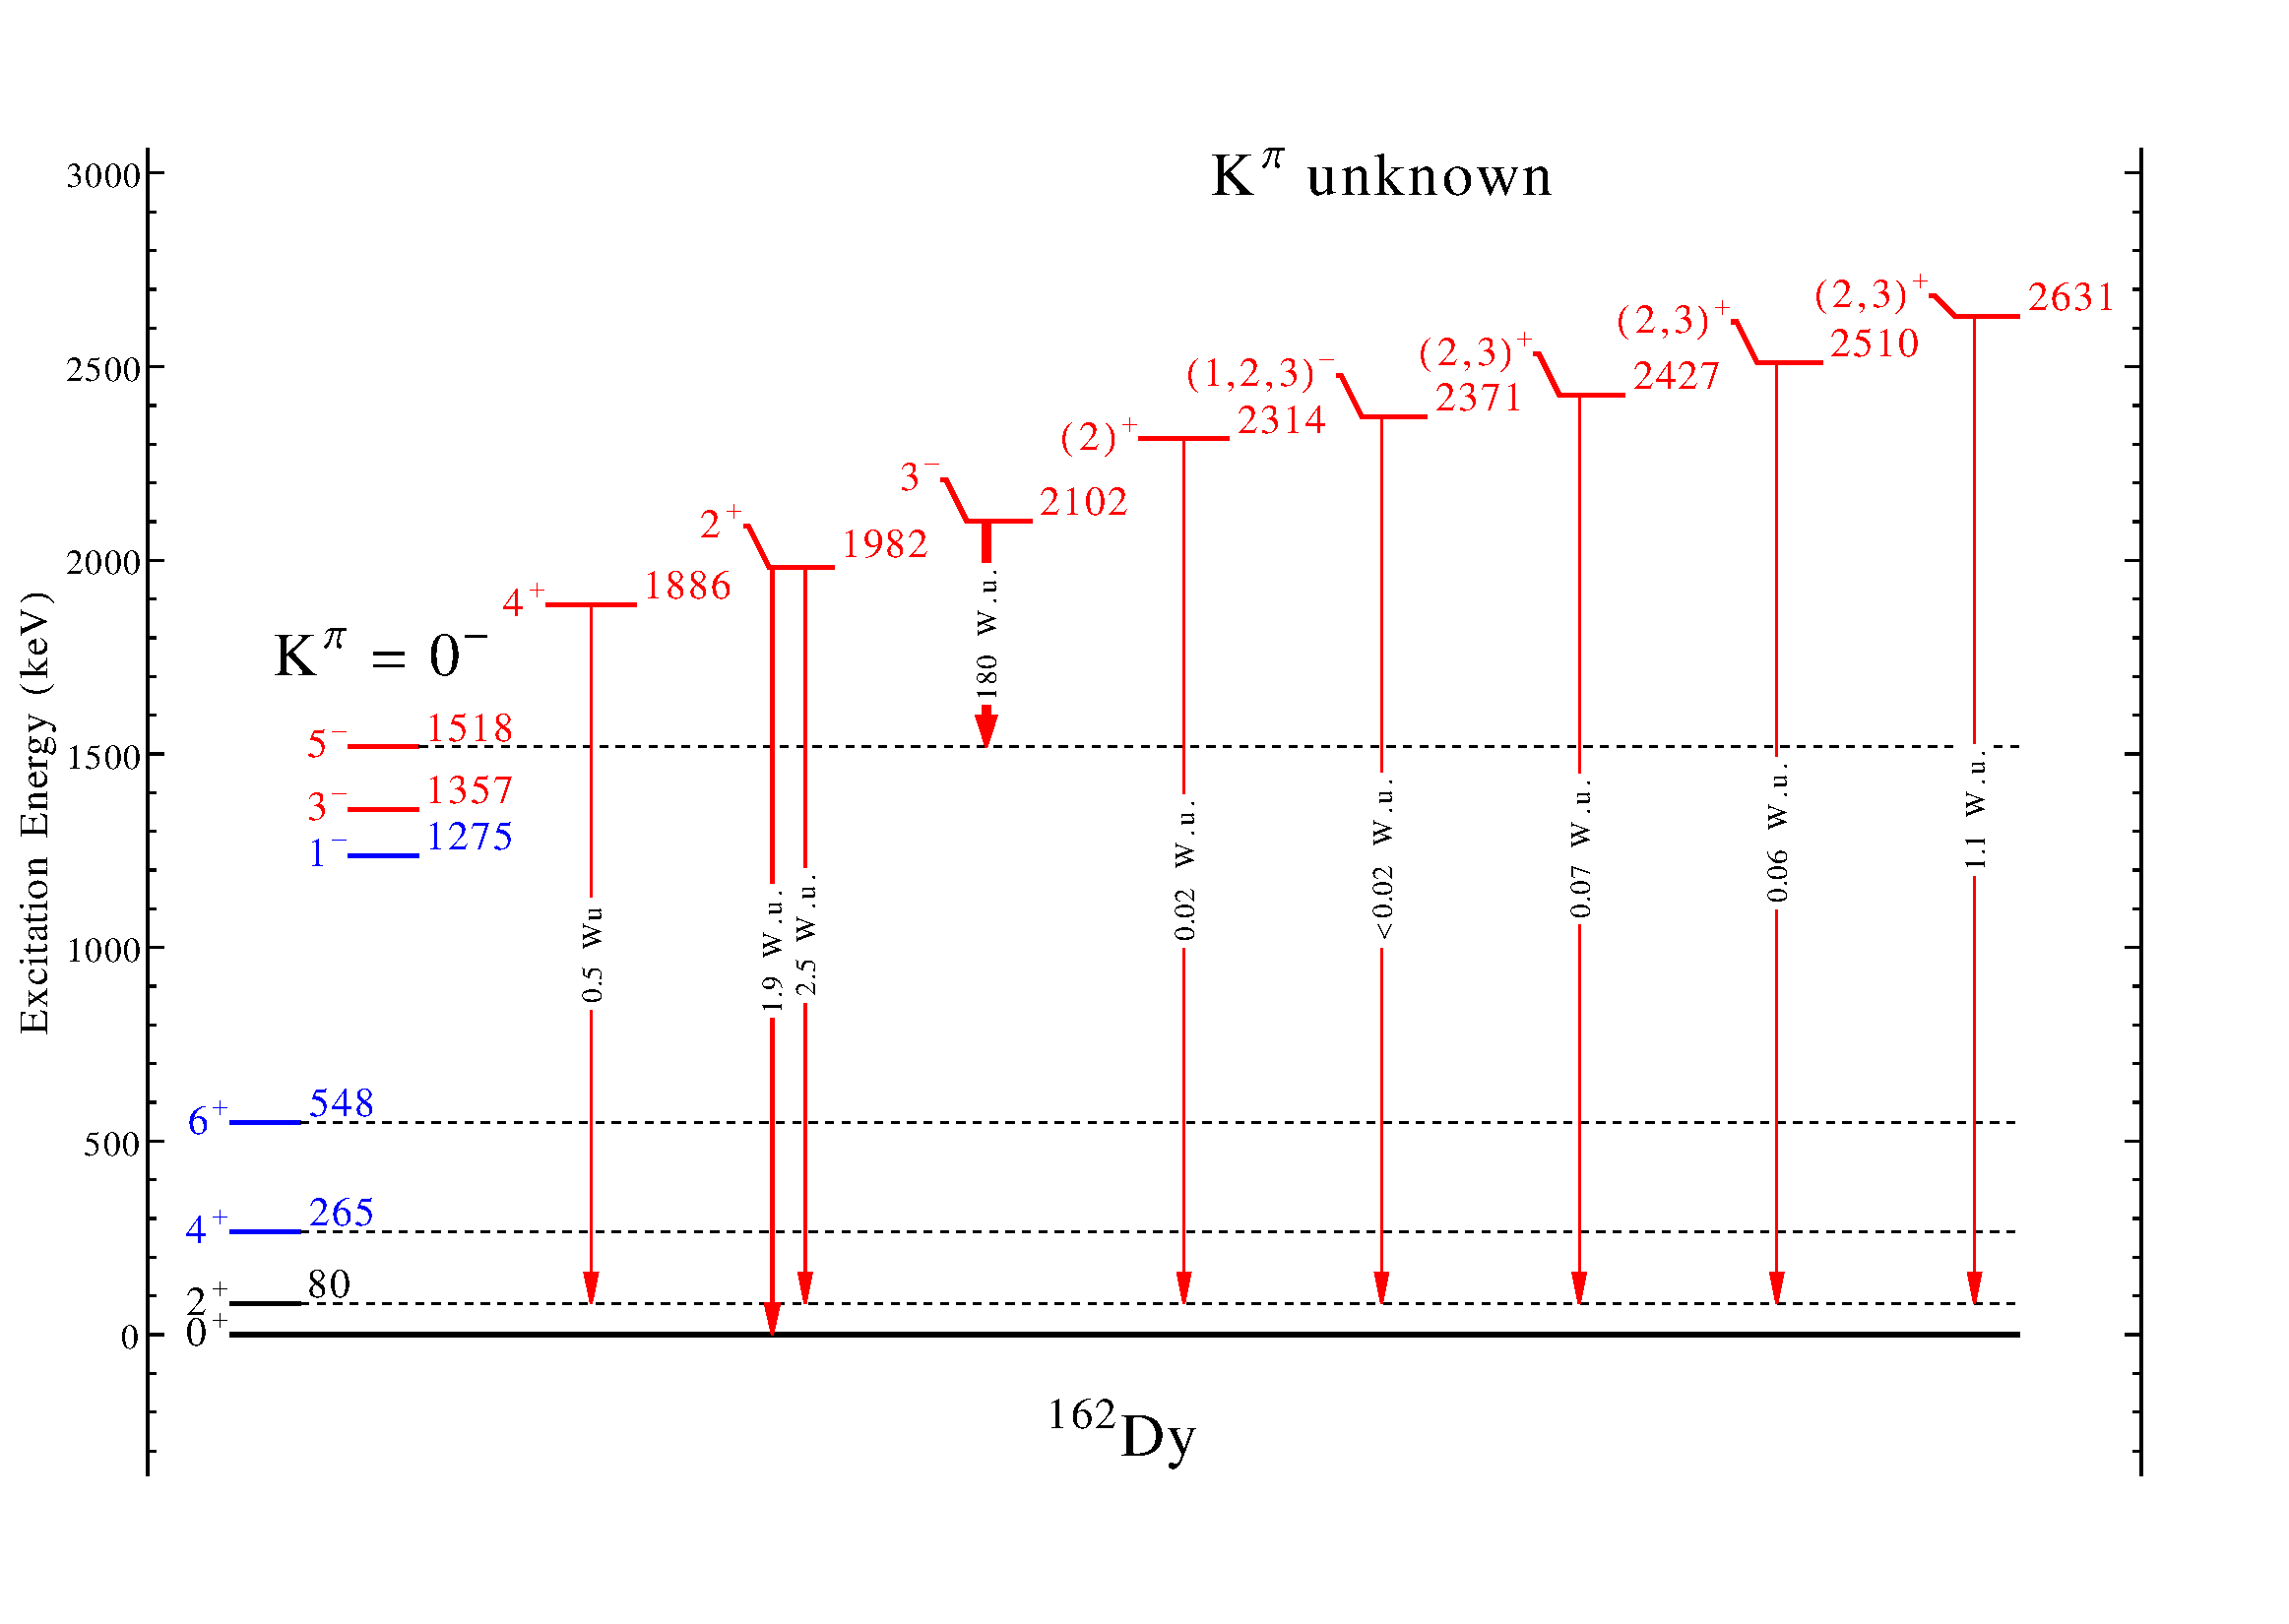
\includegraphics[height=0.85\textheight]{figures/162Dy_misc.pdf}
\end{center}
\caption{Levels in $^{162}$Dy with no rotational band assignment above the pairing gap (2$\Delta$n=1720~keV \& 2$\Delta$p=1914~keV). B(E2) strenghts drawn in red and in W.u. \label{fig:162Dy_misc}}
\end{figure}
\end{landscape}

\begin{landscape}
\begin{figure}[h!]
\begin{center}
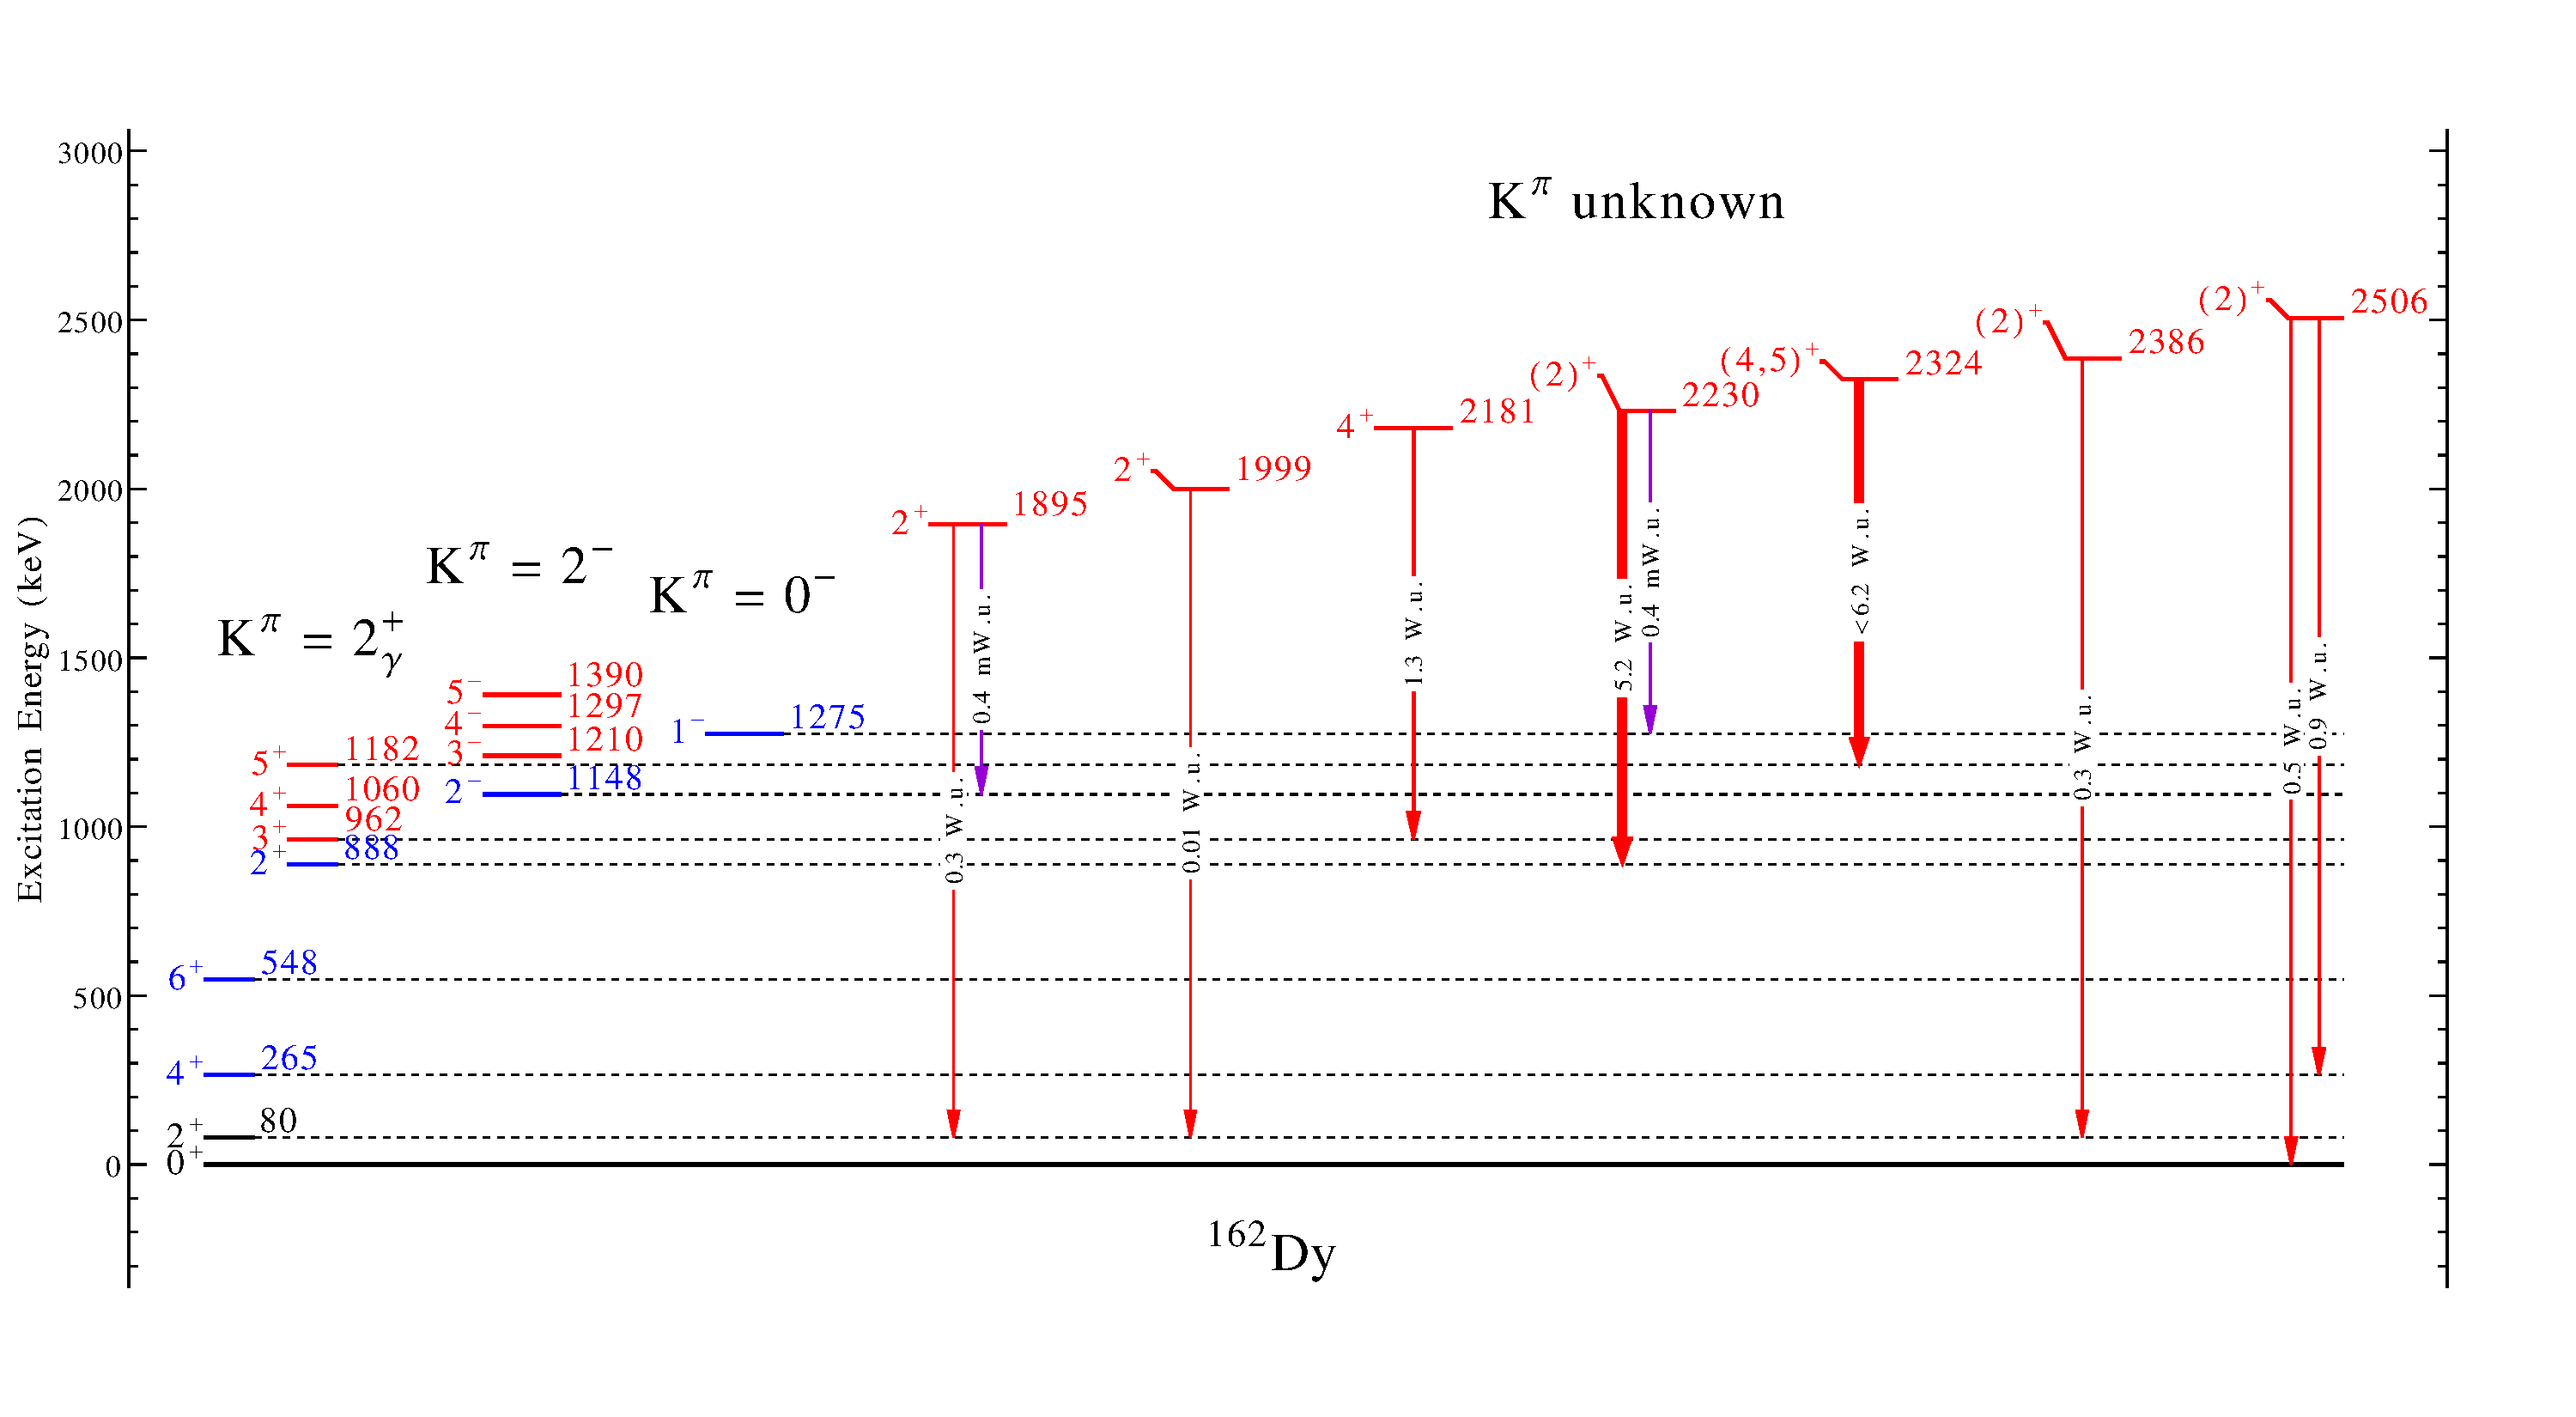
\includegraphics[height=0.85\textheight]{figures/162Dy_misc2.pdf}
\end{center}
\caption{Levels in $^{162}$Dy with no rotational band assignment above the pairing gap (2$\Delta$n=1720~keV \& 2$\Delta$p=1914~keV) (continued). B(E1) in violet and in mW.u., and B(E2) in red in W.u. \label{fig:162Dy_misc2}}
\end{figure}
\end{landscape}

\begin{landscape}
\begin{figure}[h!]
\begin{center}
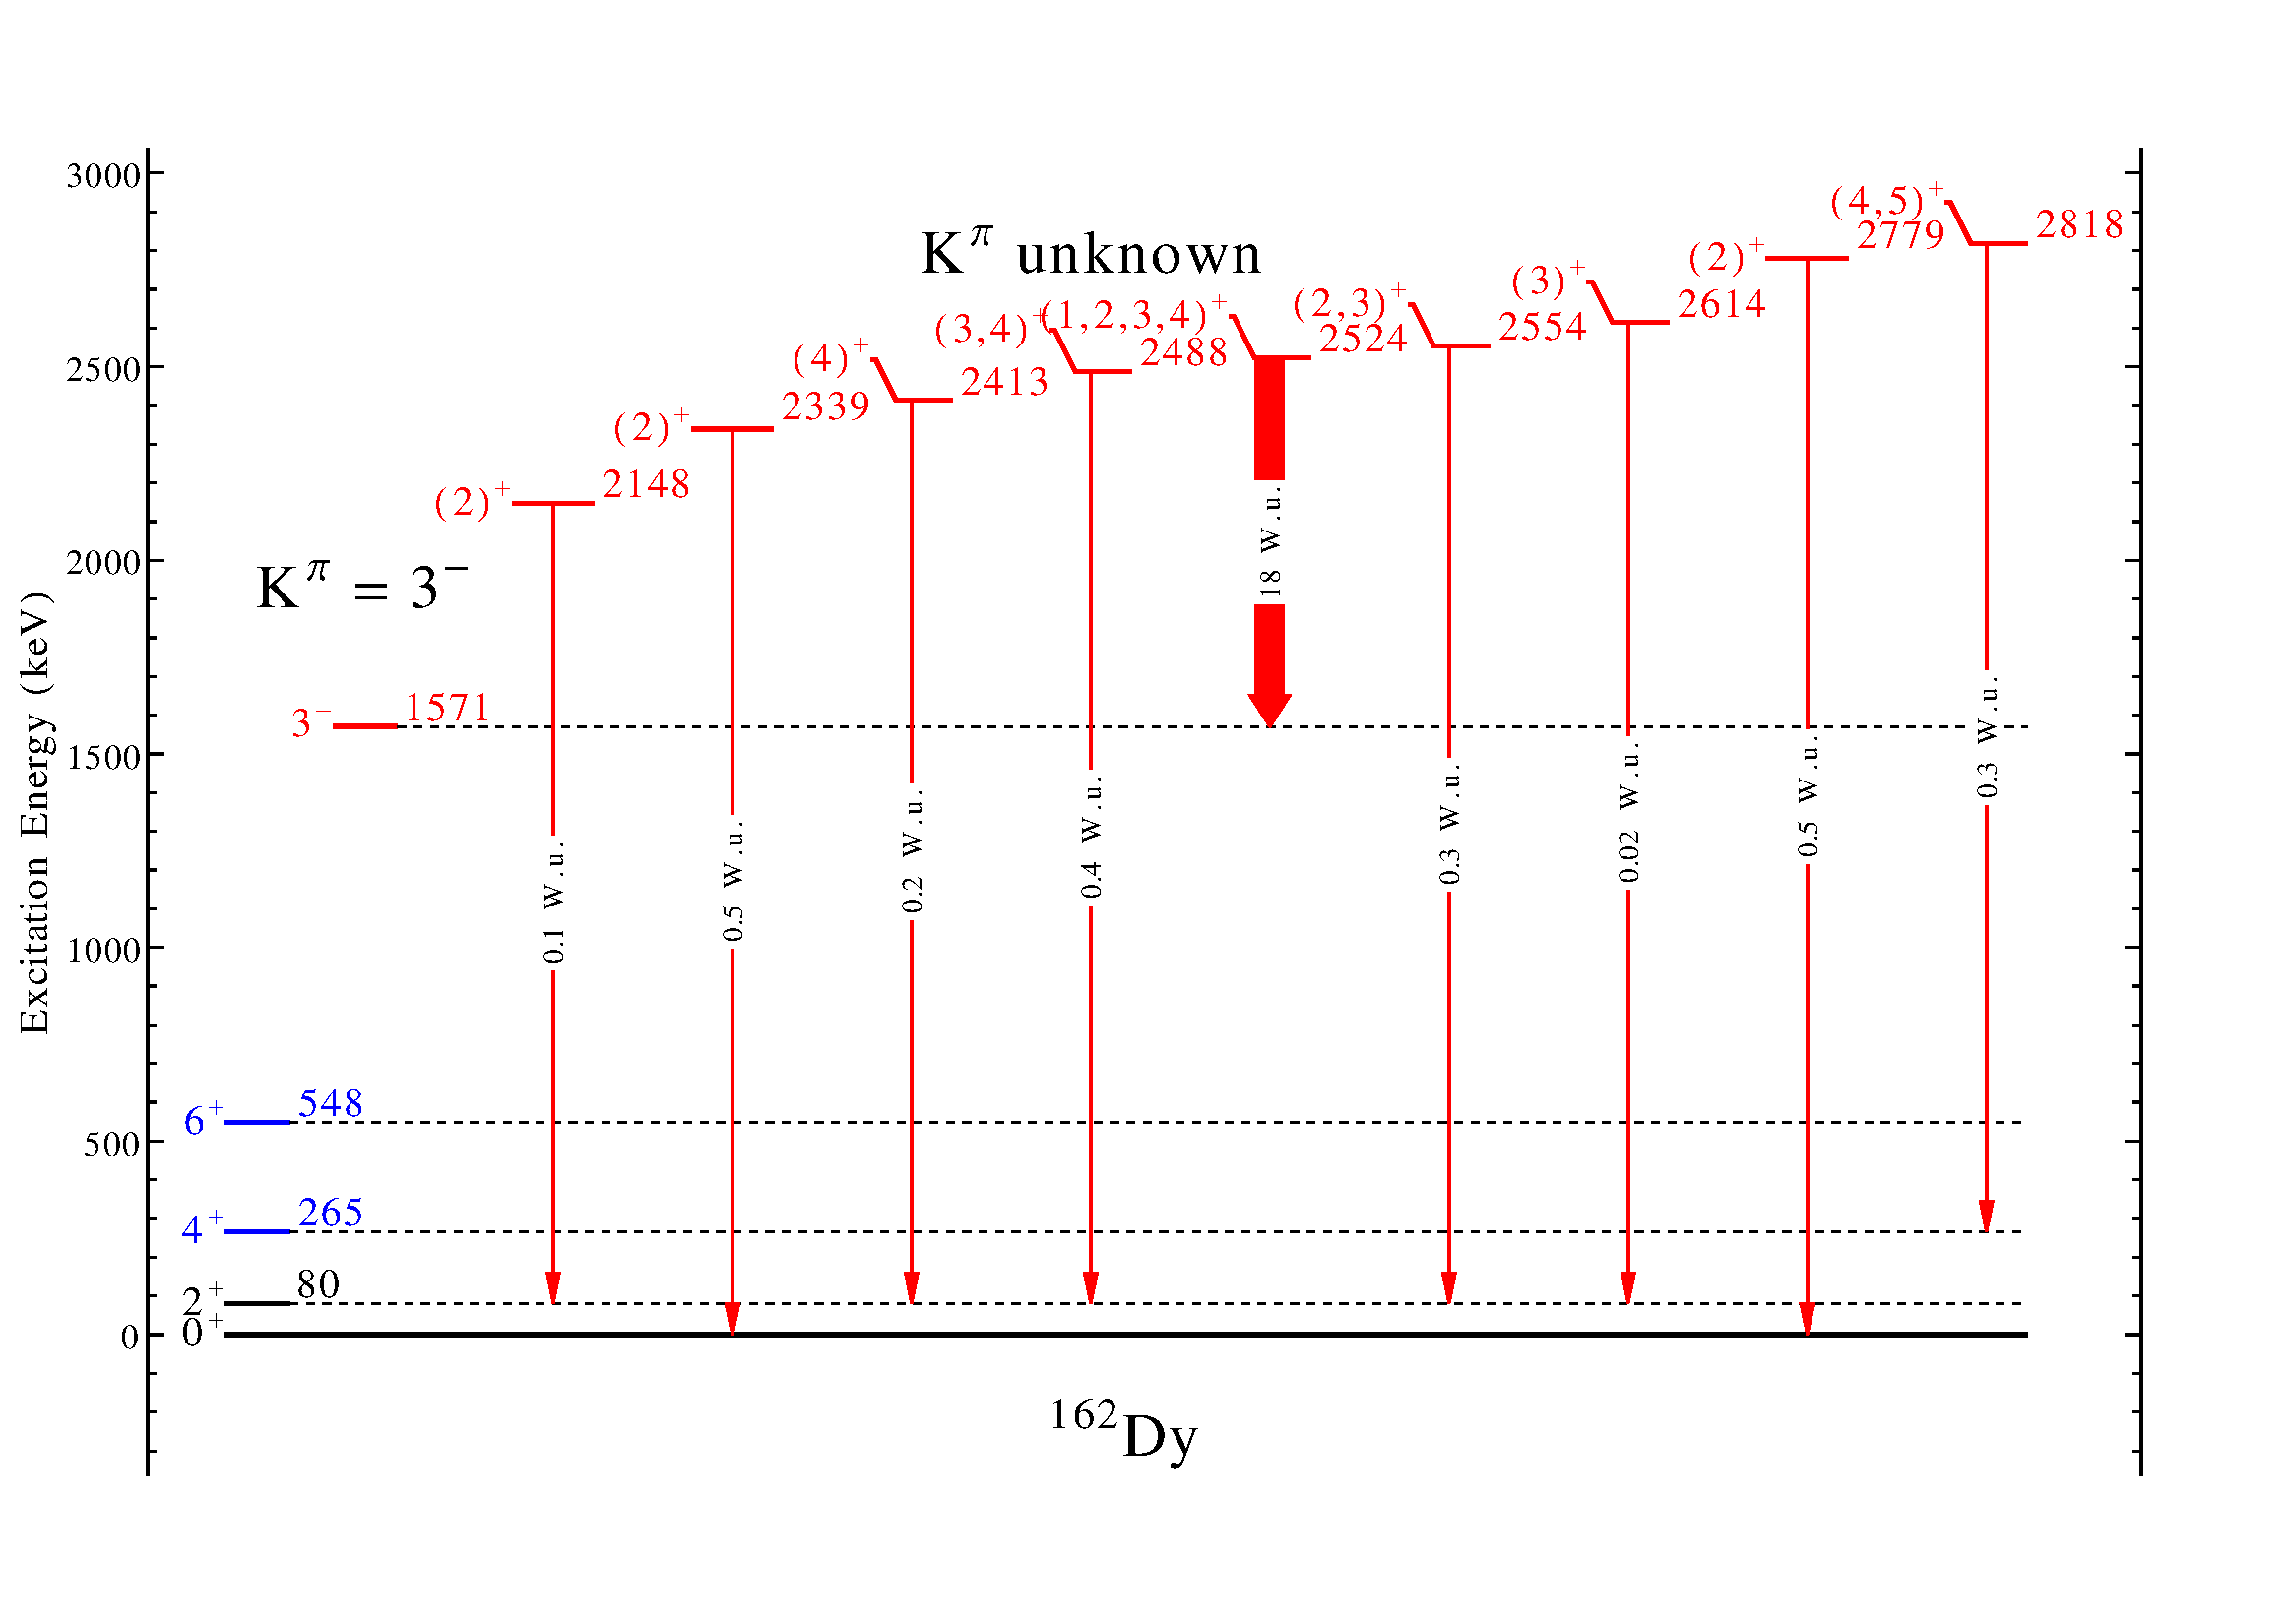
\includegraphics[height=0.85\textheight]{figures/162Dy_misc3.pdf}
\end{center}
\caption{Levels in $^{162}$Dy with no rotational band assignment above the pairing gap (2$\Delta$n=1720~keV \& 2$\Delta$p=1914~keV) (continued). B(E1) in violet and in mW.u., and B(E2) in red in W.u. \label{fig:162Dy_misc}}
\end{figure}
\end{landscape}


\subsection{Implications and Further Discussion}
Lifetime measurements for $^{162}$Dy offer a remarkable survey of nuclear structure in this deformed nucleus. The definitive existence of single- and double-phonon quadrupole vibrations at the excitation energies E$_{K^\pi=2^+_\gamma}$=888~keV, E$_{K^\pi=0^+_{\gamma\gamma}}$=1400~keV, E$_{K^\pi=4^+_{1,\gamma\gamma}}$=1535~keV, E$_{K^\pi=4^+_{2,\gamma\gamma}}$=2181~keV has set a new precedent for anharmonic quadrupole vibrations, as the majority of two-phonon cases in deformed rare-earth nuclei are at higher energies than a purely harmonic case. A new opening for a potential collective state built on-top of the $\gamma$-vibrational band has been proposed as a candidate for a $\beta\gamma$-vibration, an excitation that has eluded experimentalists for years.

In a trend that continues throughout the rare-earth nuclei, lifetimes have been measured for only a few negative parity states that are surmised to be a part of the octupole vibrational states. The new decay patterns for the negative parity states in 2$^-\rightarrow$2$^+_\gamma$ transitions has been observed in our campaign of lifetime measurements, via strong E1 transitions to the $\gamma$-band. These measured K$^\pi$=2$^-$ bands seem to not be a part of the octupole vibration, but it cannot be solidified without precision B(E3) measurements in the interband cases; whether or not these states are a separate collective degree of freedom besides the traditional quadrupole/octupole vibration remains an open question.


% }